\clearpage
\section{Validation of the QCD prediction \label{app:qcdPredictionValidation}}

Fig.~\ref{fig:RR_qcd} illustrates the Validation of the QCD prediction method with data-driven measurements. Figs.~\ref{fig:asym_qcd_validation}-\ref{fig:asym_qcd_validation} illustrate the agreement between QCD and electroweak shapes in $\nb$ and \mht.

\begin{figure}[h!]
  \begin{center}        
    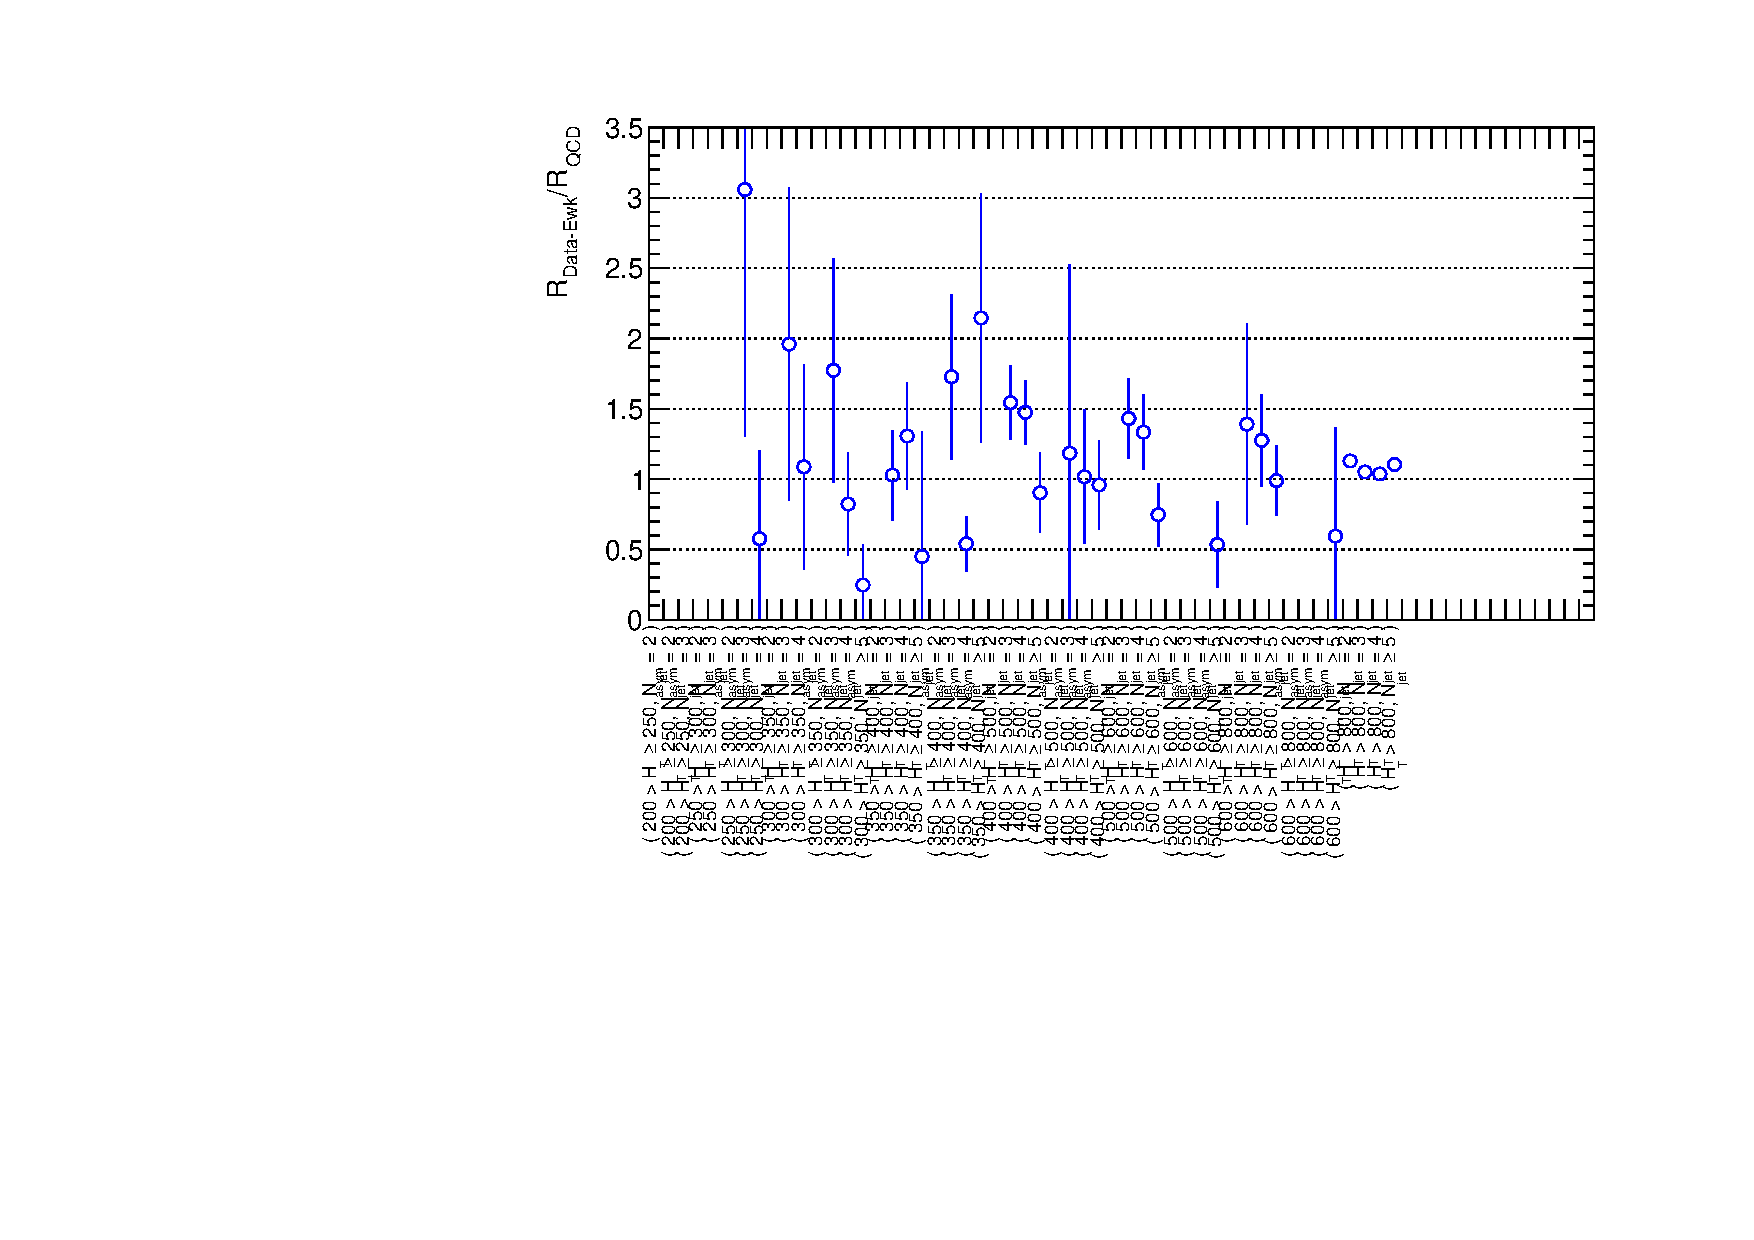
\includegraphics[width=\textwidth]{figures/qcd/validation/RRPlot}
    \caption{ Ratio of the measurement of \rmhtmet, the pass/fail ratio for the \mhtmet selection, from data and Monte Carlo in the $\bdphi < 0.5$ sideband in (\scalht, \njet) bins.  
    }

    \label{fig:RR_qcd}
  \end{center} 
\end{figure}


\begin{figure}[h!]
  \begin{center}
    \subfigure[{ Asymmetric, $\scalht<400$~GeV}]{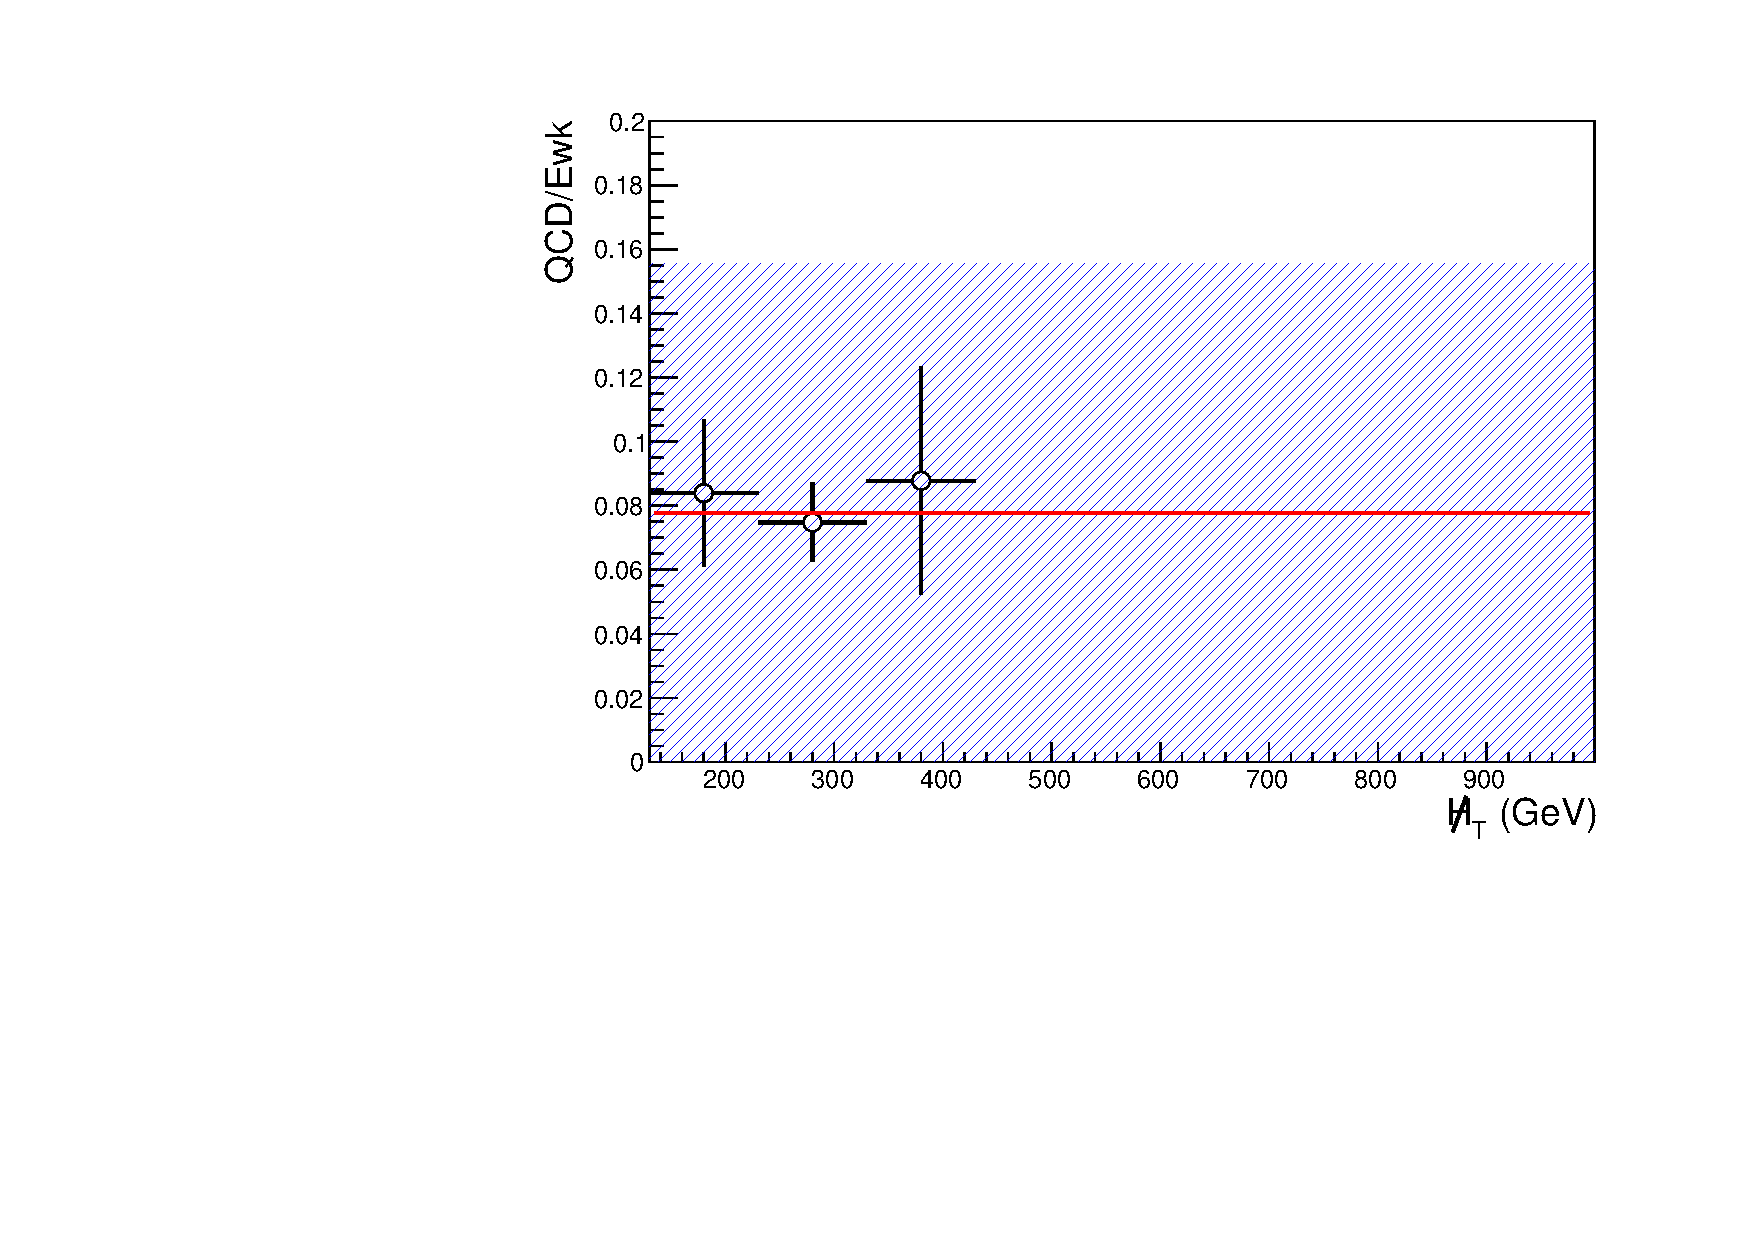
\includegraphics[width=0.5\textwidth]{figures/qcd/validation/Ratio_Asym_HTlt400_mht}} ~~
    \subfigure[{ Asymmetric, $\scalht<400$~GeV}]{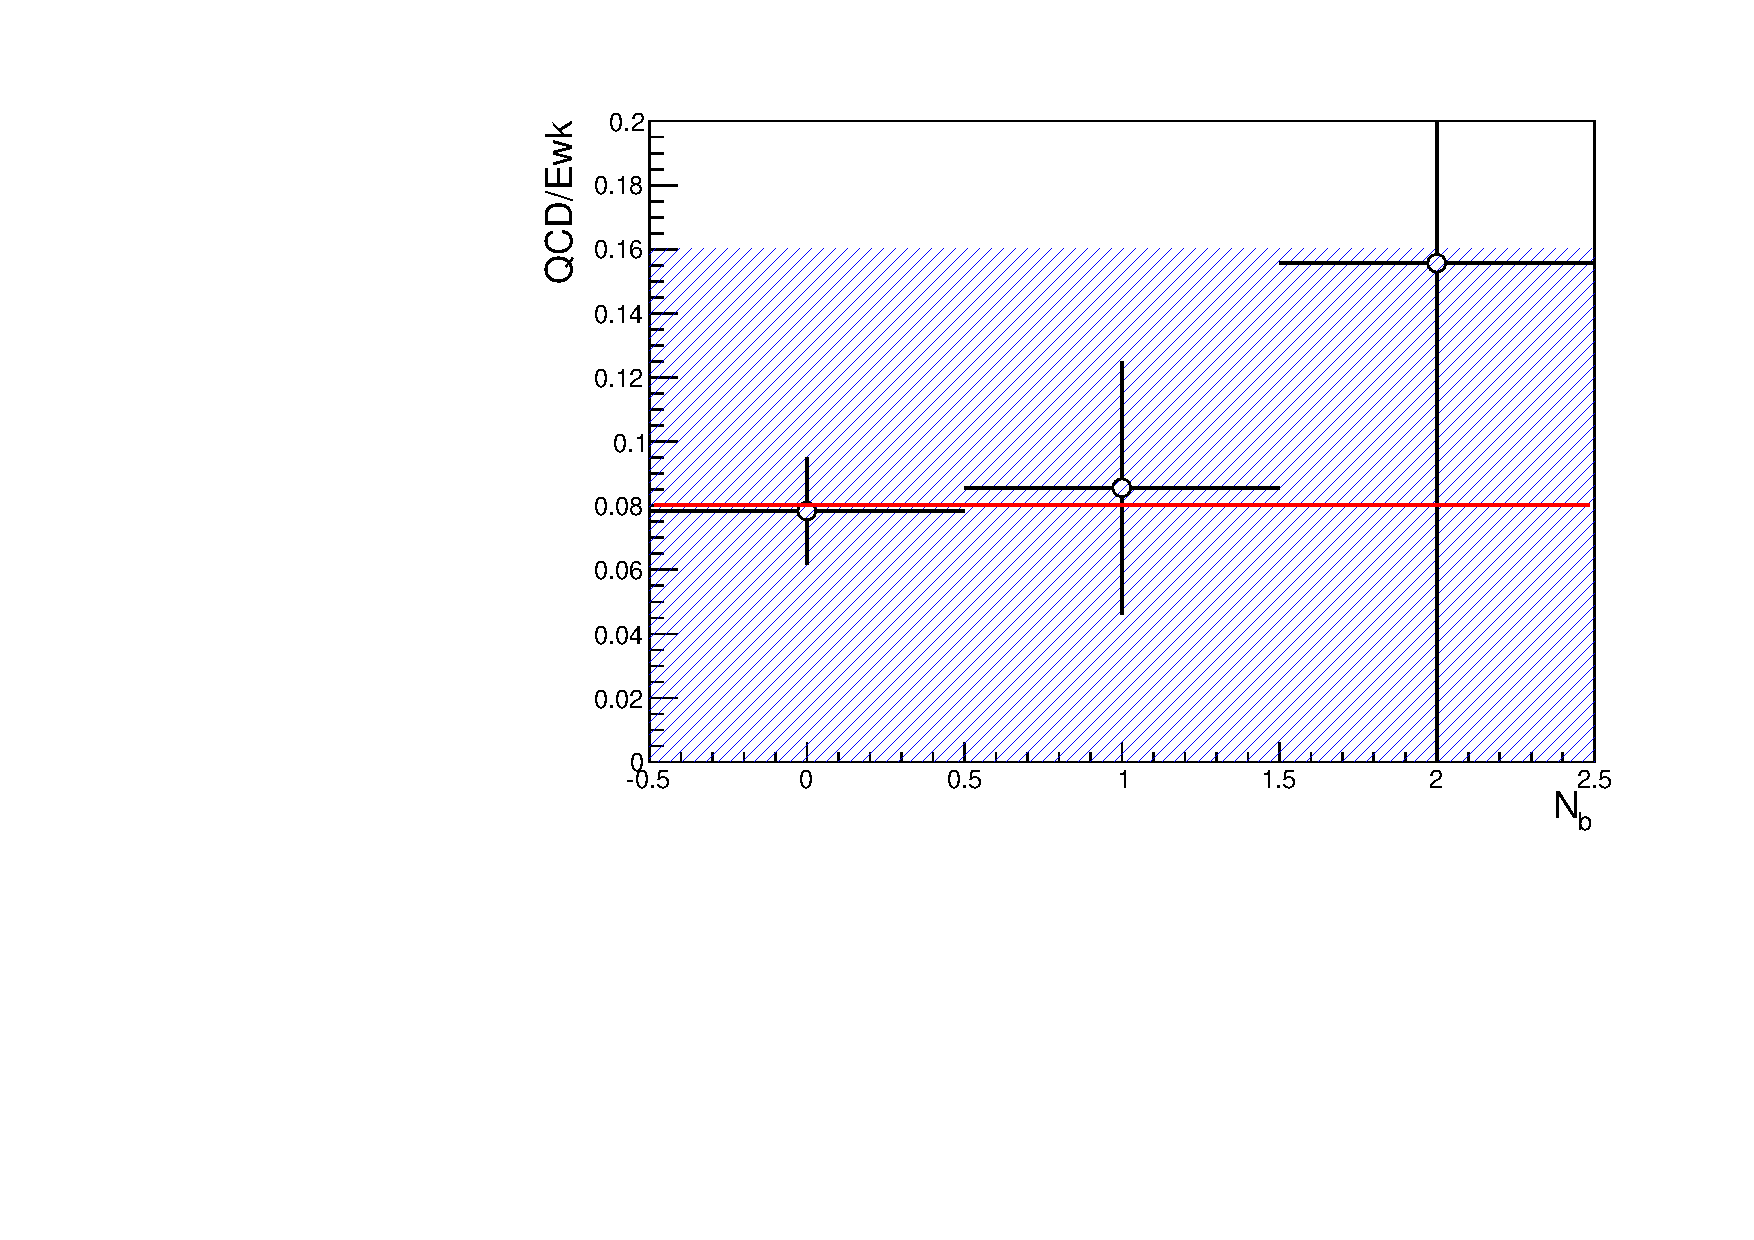
\includegraphics[width=0.5\textwidth]{figures/qcd/validation/Ratio_Asym_HTlt400_nB}} \\
    \subfigure[{ Asymmetric, $\scalht>400$~GeV}]{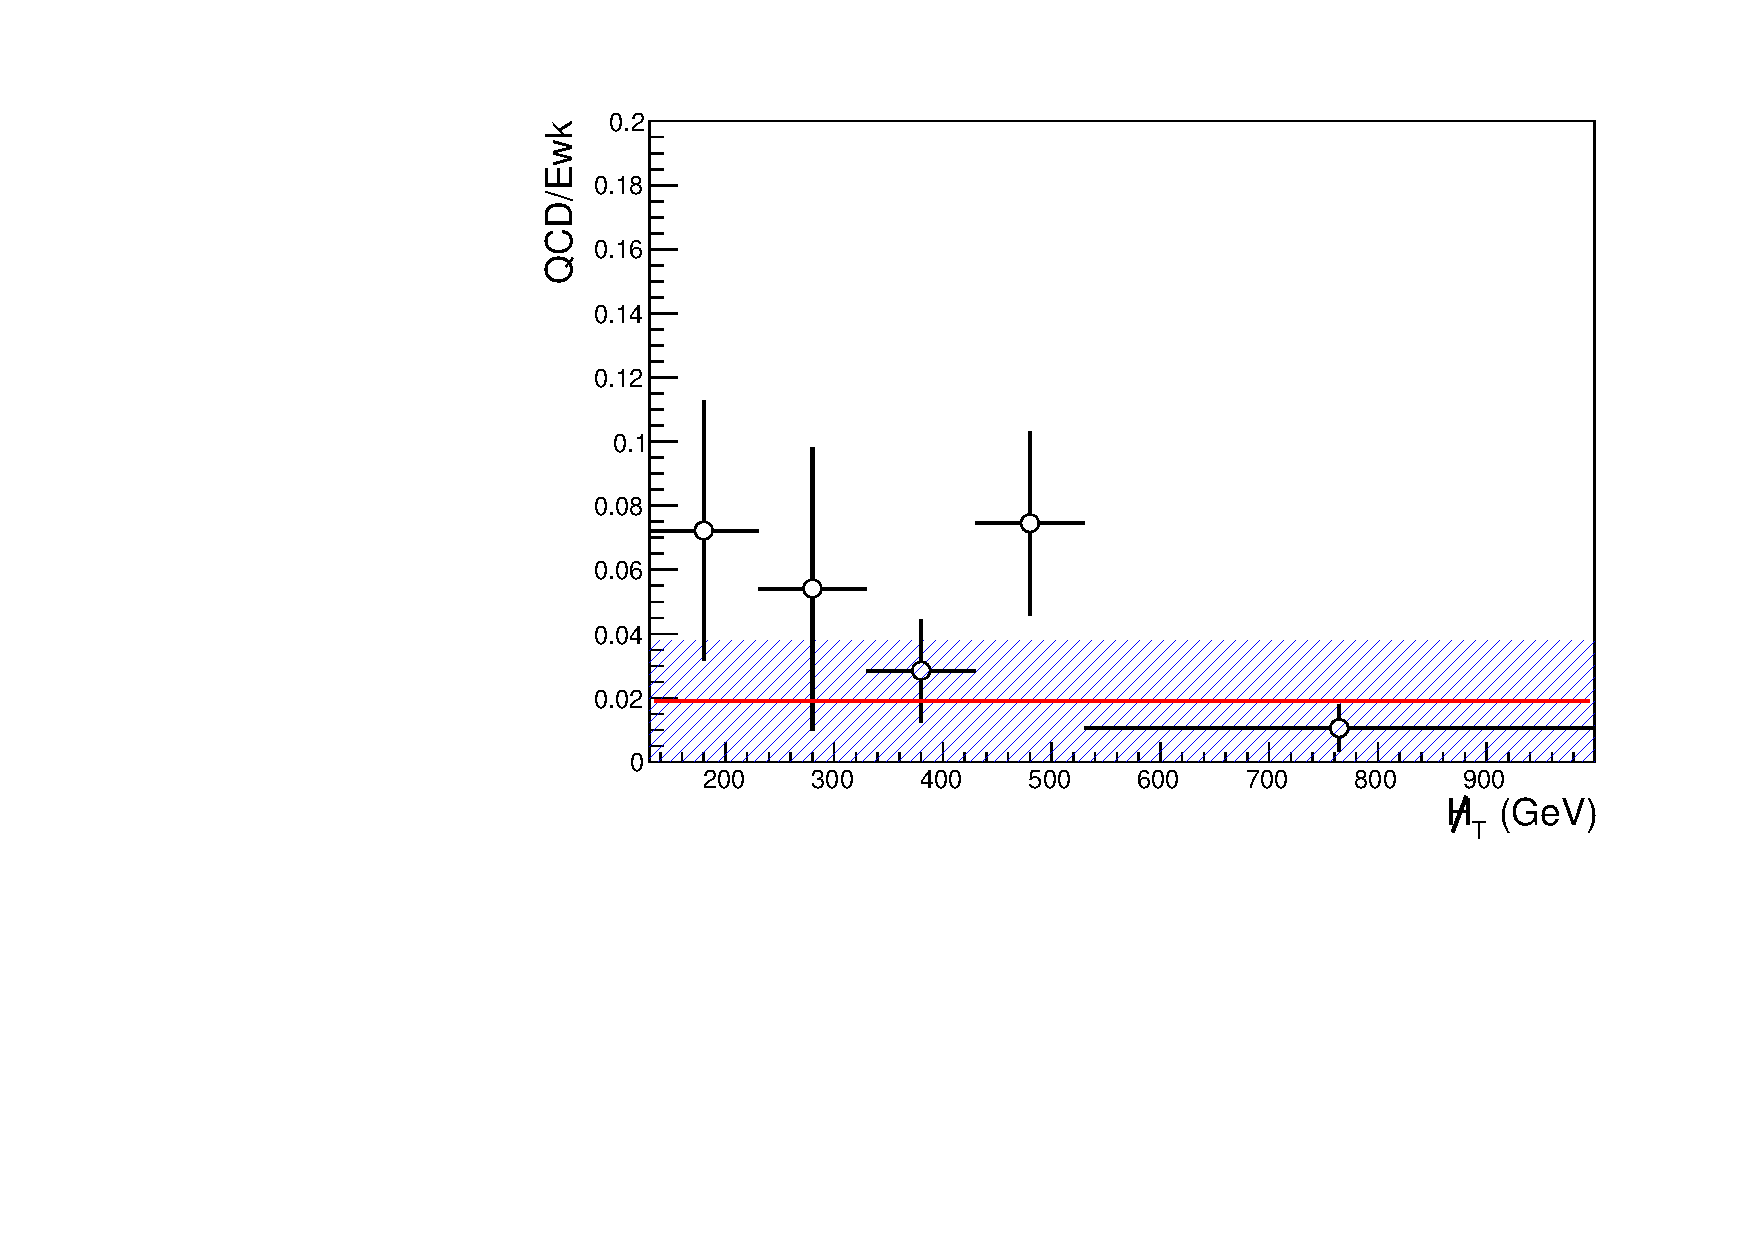
\includegraphics[width=0.5\textwidth]{figures/qcd/validation/Ratio_Asym_HTgt400_mht}} ~~
    \subfigure[{ Asymmetric, $\scalht>400$~GeV}]{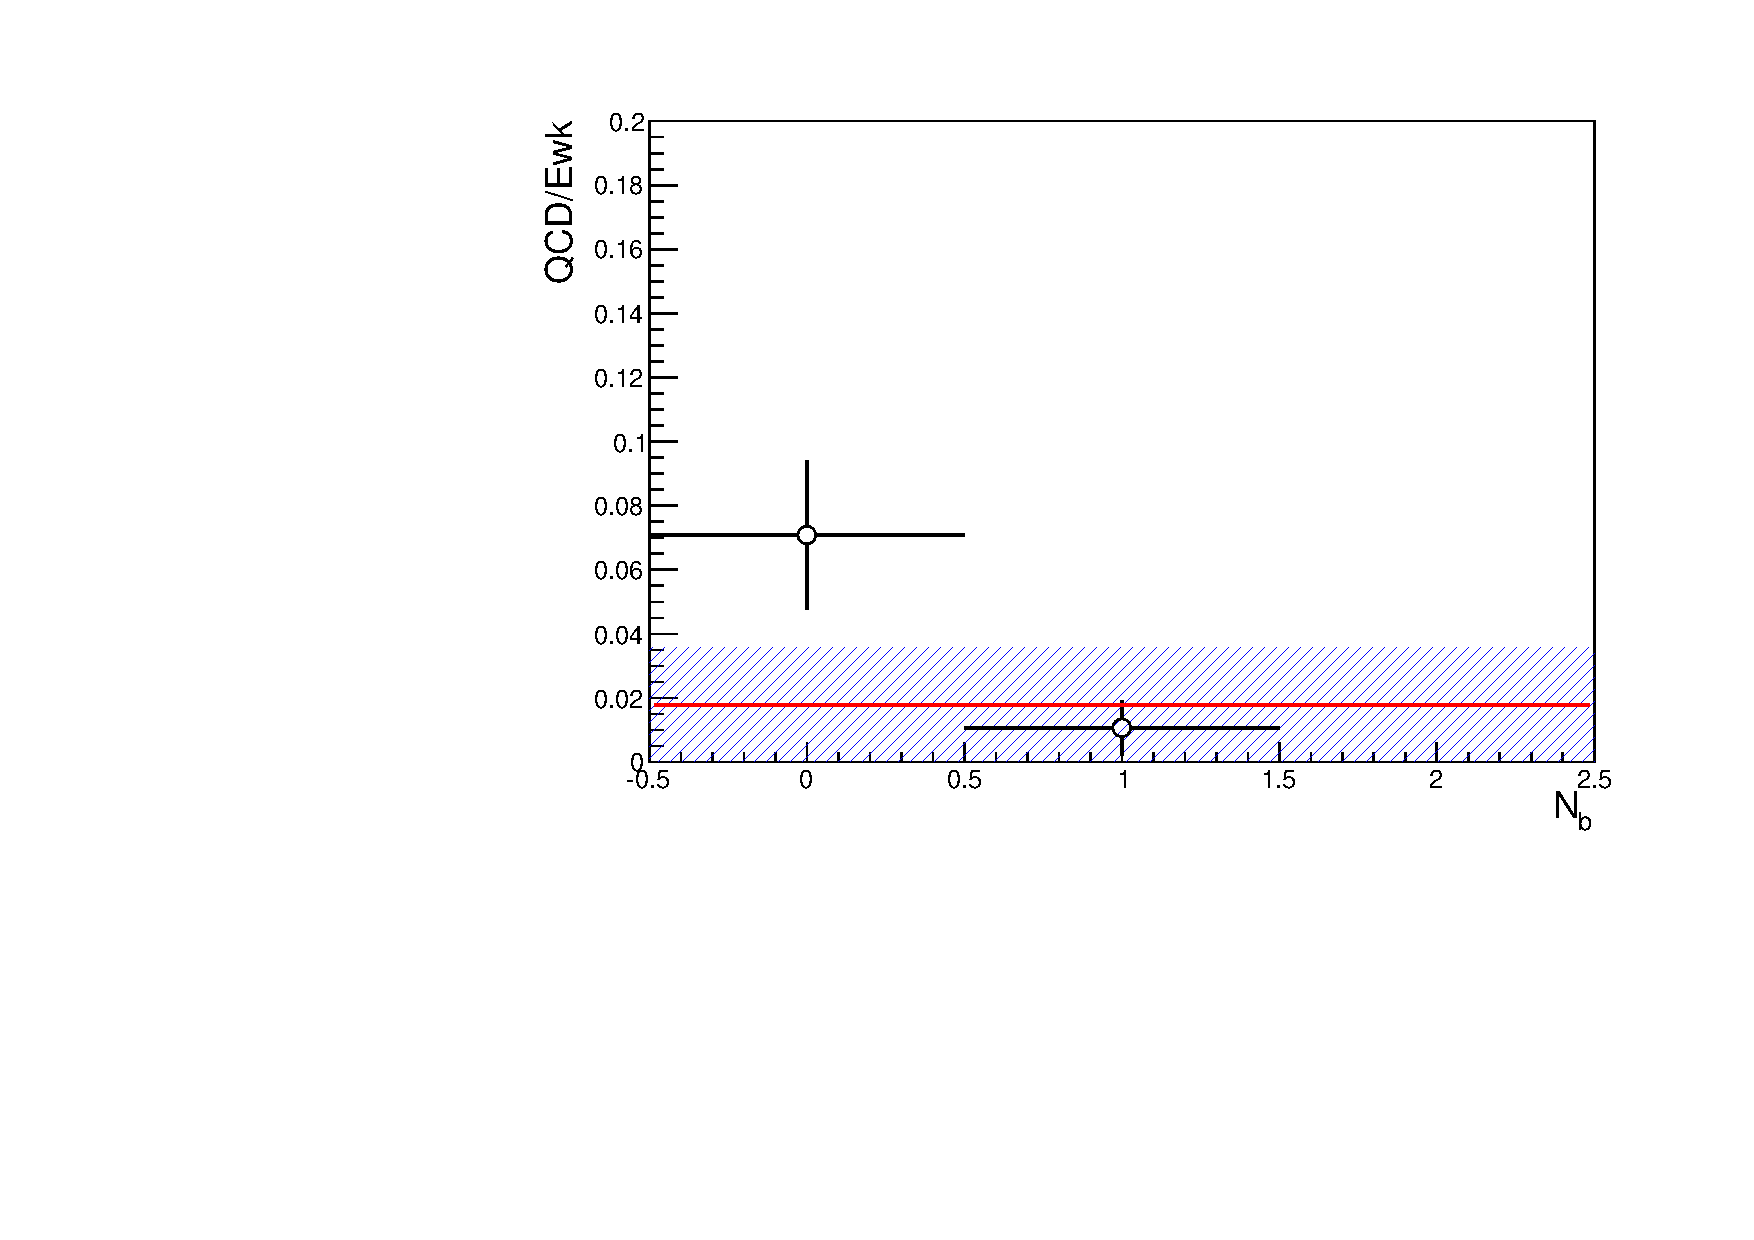
\includegraphics[width=0.5\textwidth]{figures/qcd/validation/Ratio_Asym_HTgt400_nB}} \\
    \caption{ Ratio of QCD to electroweak Monte Carlo prediction in the signal region for different \scalht selections as a function of \mht (Left) and $\nb$ (Right) for the asymmetric jet category. A constant fit to the data is represented by the red line, with the $\pm$100\% uncertainty represented by the blue hashed region.
    }
    \label{fig:asym_qcd_validation}
  \end{center} 
\end{figure}


\clearpage
\begin{figure}[h!]
  \begin{center}
    \subfigure[{ Symmetric, $\scalht<400$~GeV}]{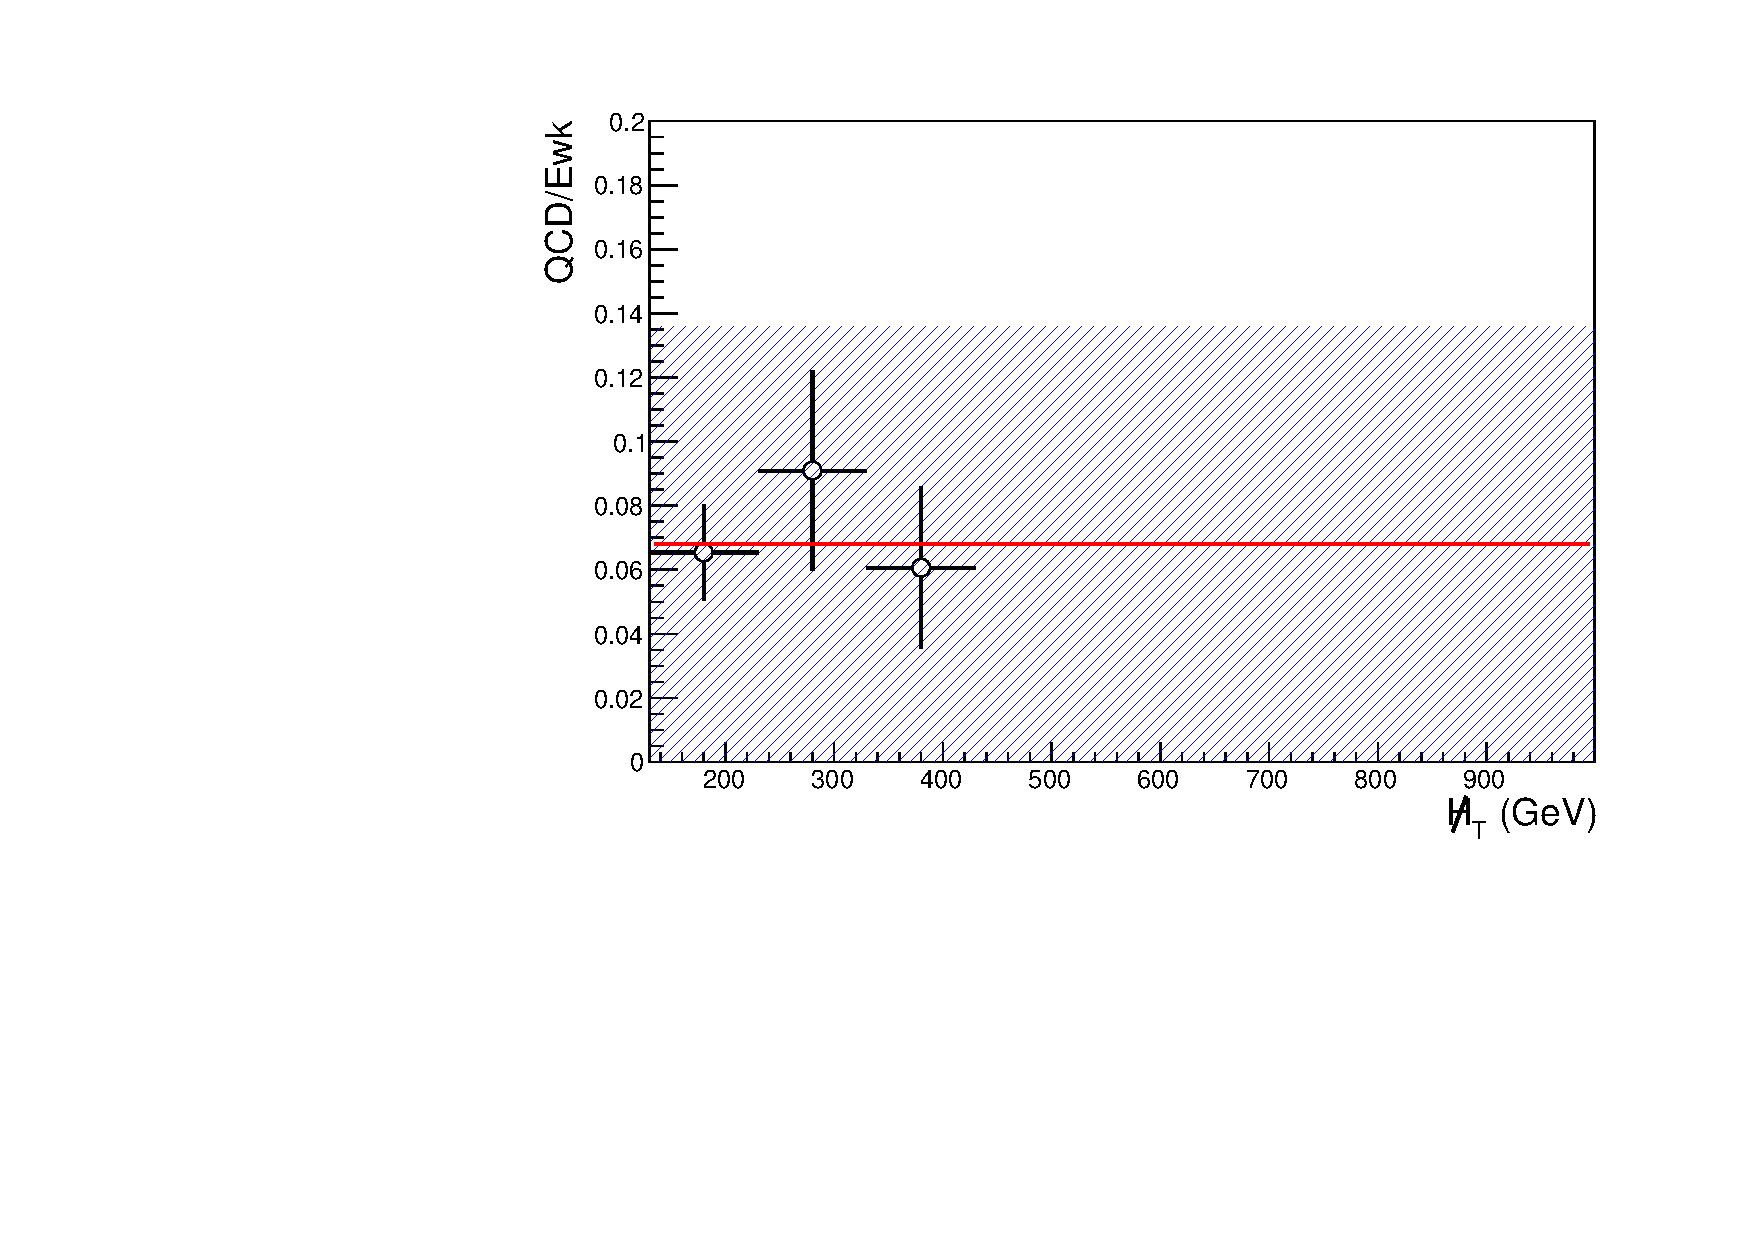
\includegraphics[width=0.5\textwidth]{figures/qcd/validation/Ratio_Sym_HTlt400_mht}} ~~
    \subfigure[{ Symmetric, $\scalht<400$~GeV}]{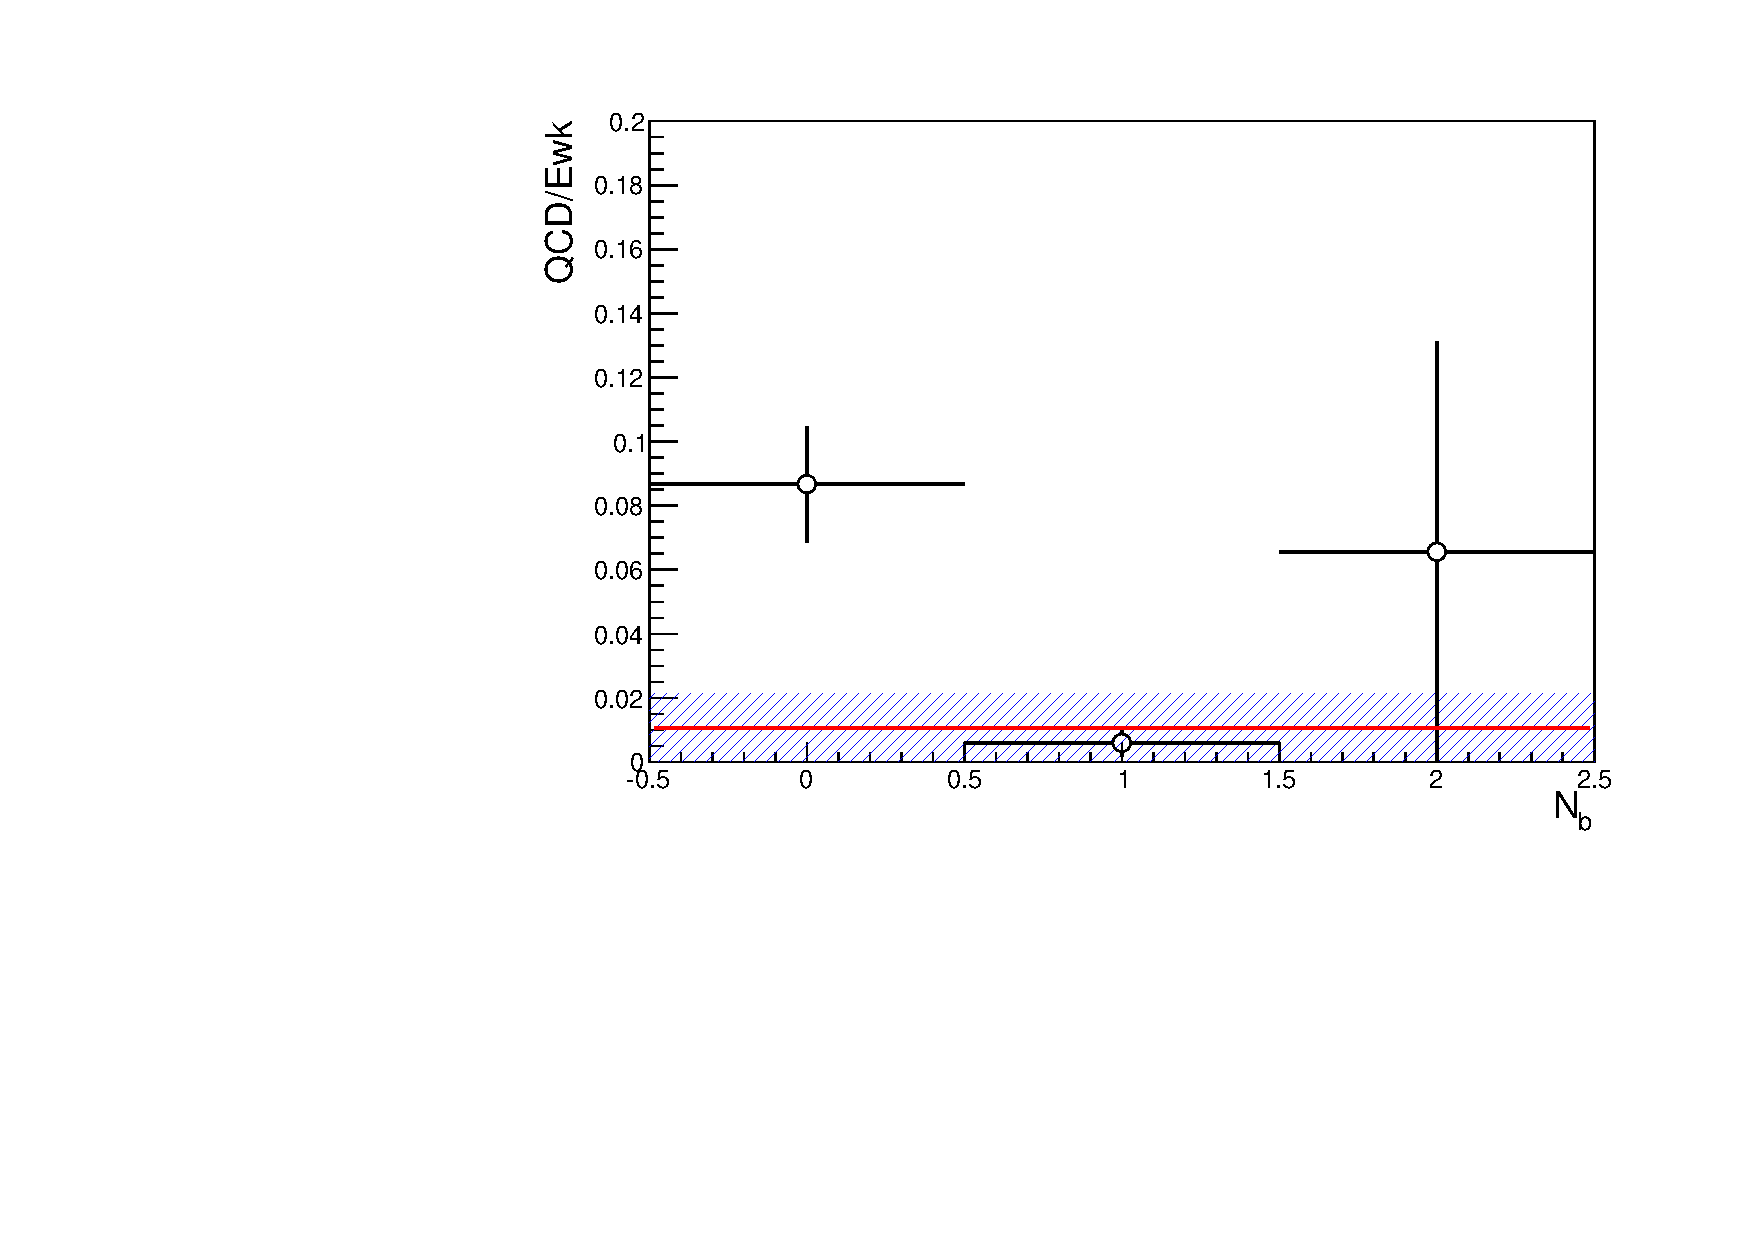
\includegraphics[width=0.5\textwidth]{figures/qcd/validation/Ratio_Sym_HTlt400_nB}} \\
    \subfigure[{ Symmetric, $\scalht>400$~GeV}]{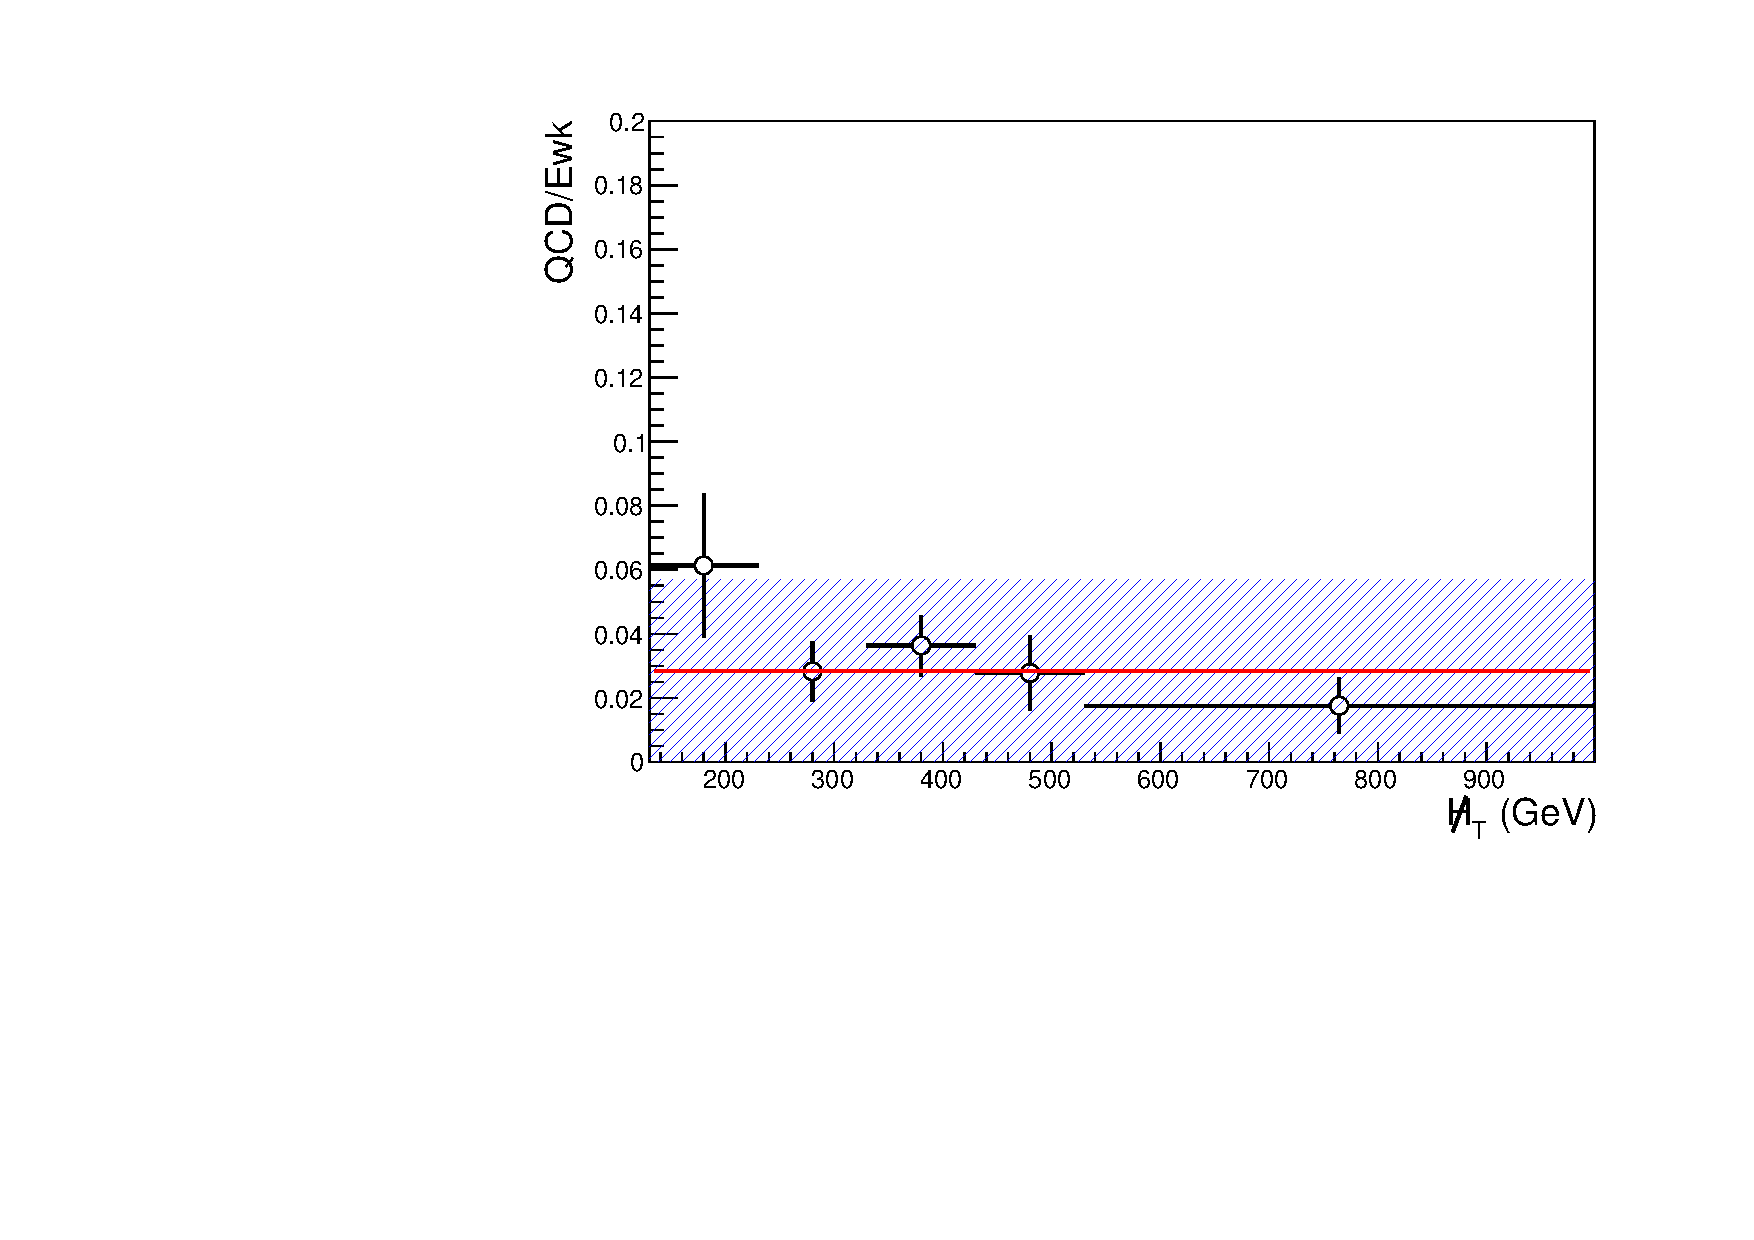
\includegraphics[width=0.5\textwidth]{figures/qcd/validation/Ratio_Sym_HTgt400_mht}} ~~
    \subfigure[{ Symmetric, $\scalht>400$~GeV}]{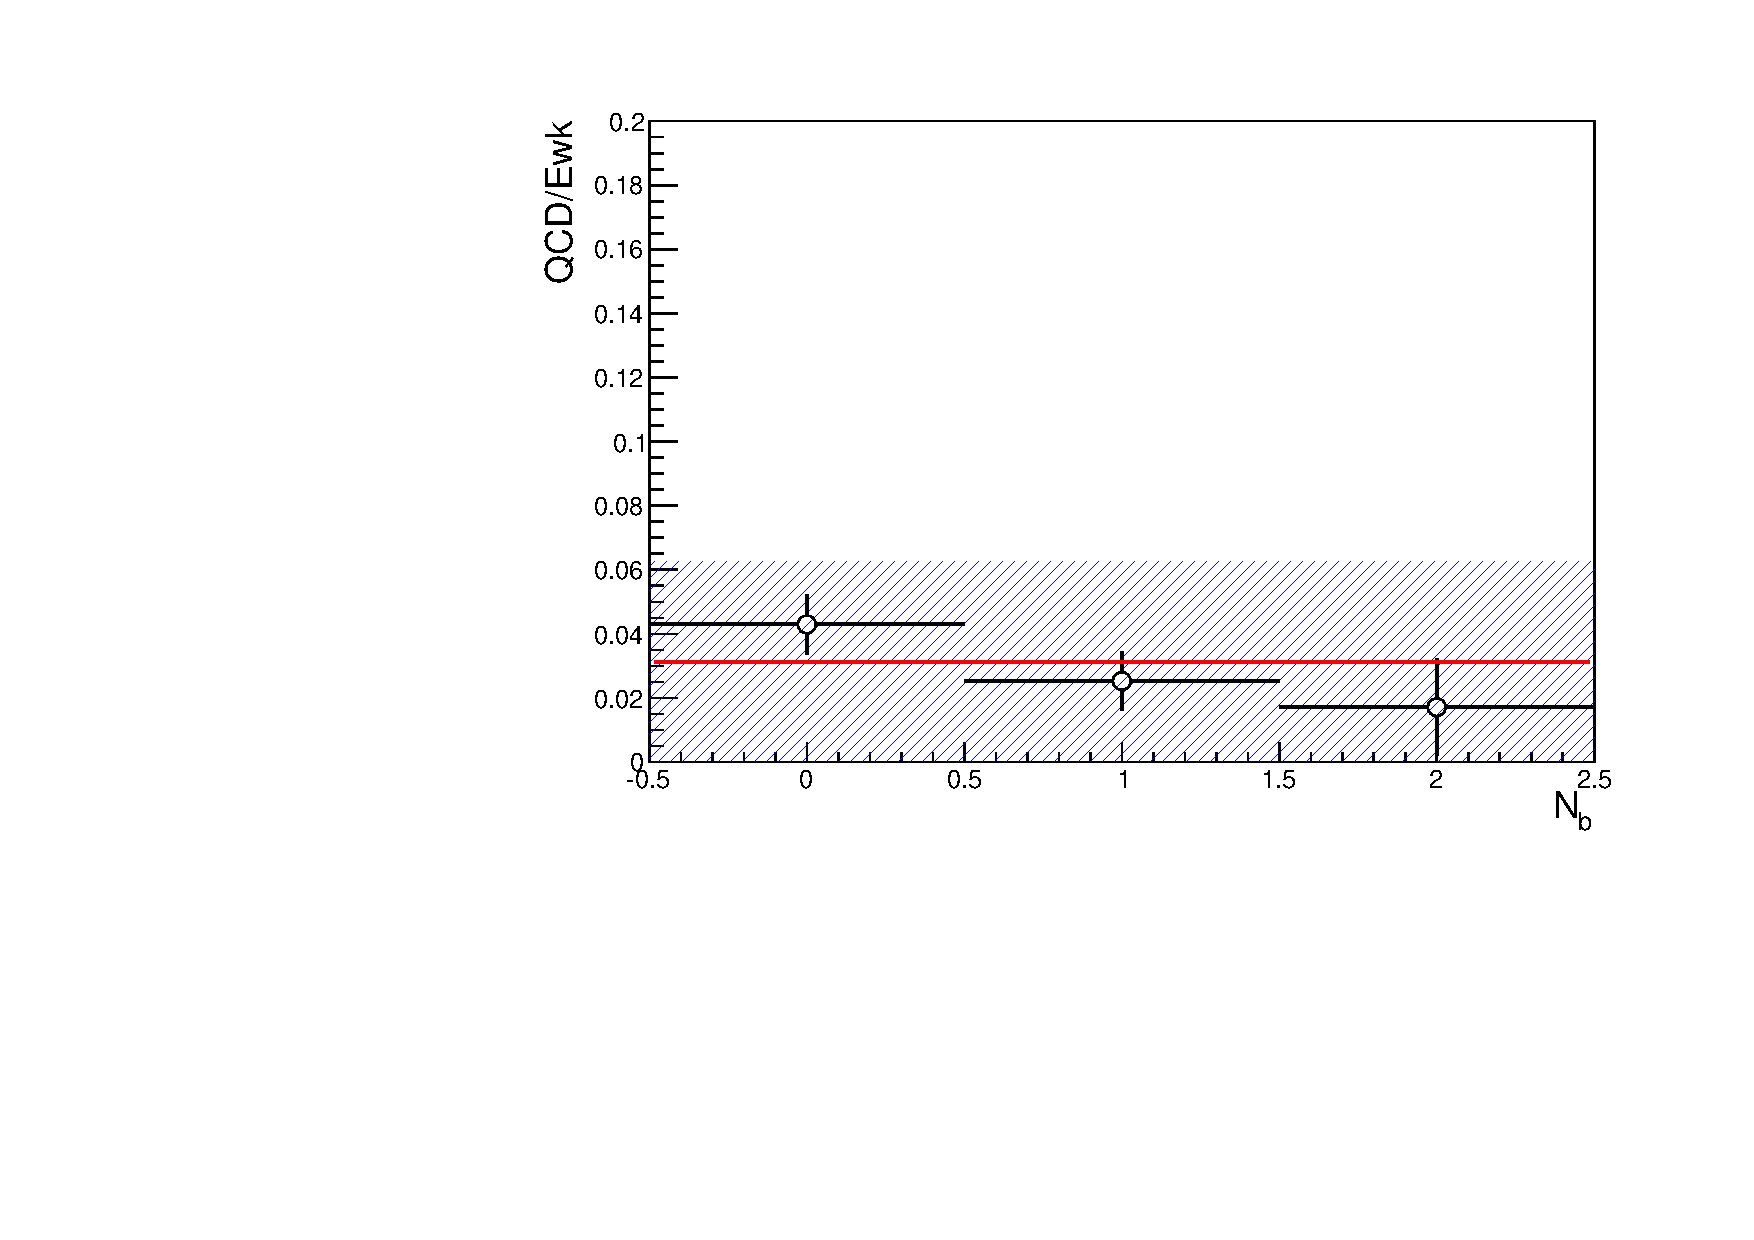
\includegraphics[width=0.5\textwidth]{figures/qcd/validation/Ratio_Sym_HTgt400_nB}} \\
    \subfigure[{ Symmetric, $\scalht>800$~GeV}]{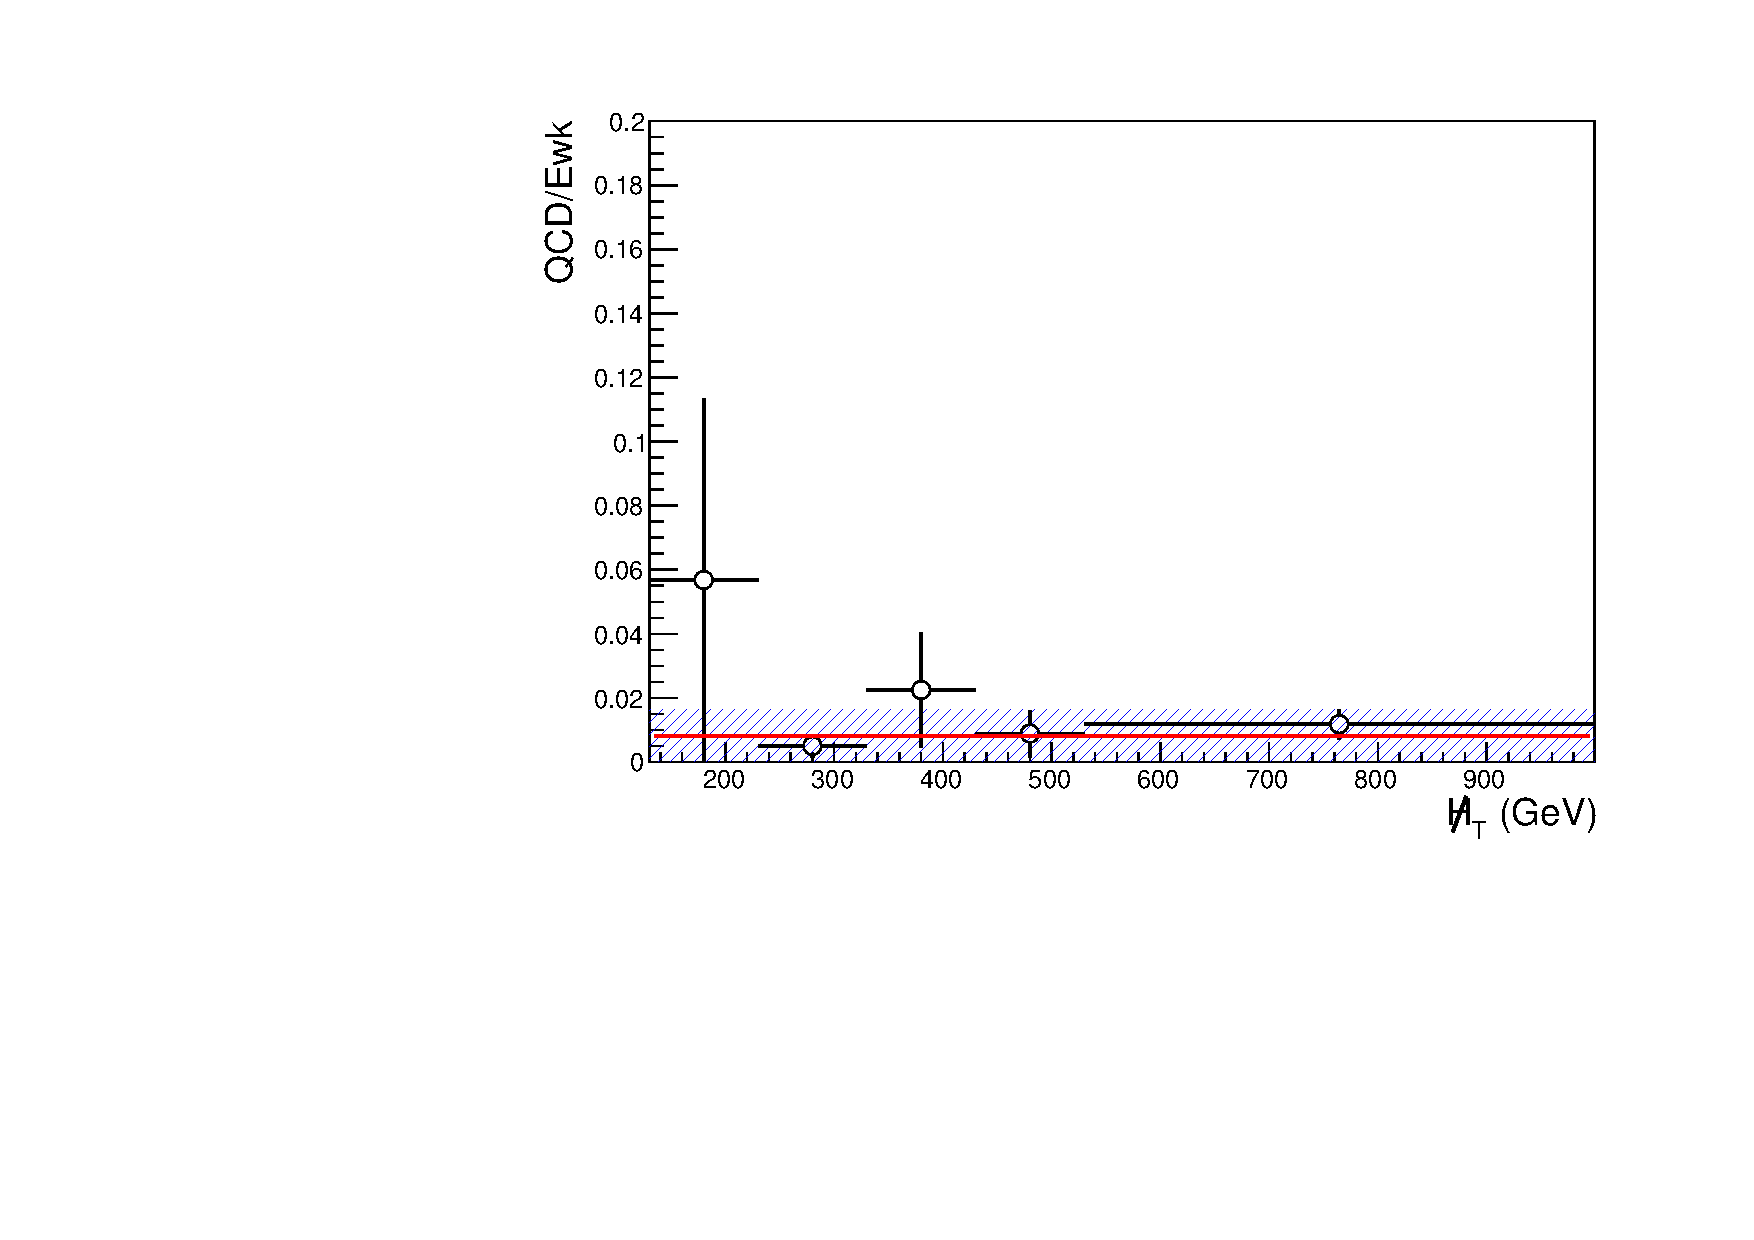
\includegraphics[width=0.5\textwidth]{figures/qcd/validation/Ratio_Sym_HTgt800_mht}} ~~
    \subfigure[{ Symmetric, $\scalht>800$~GeV}]{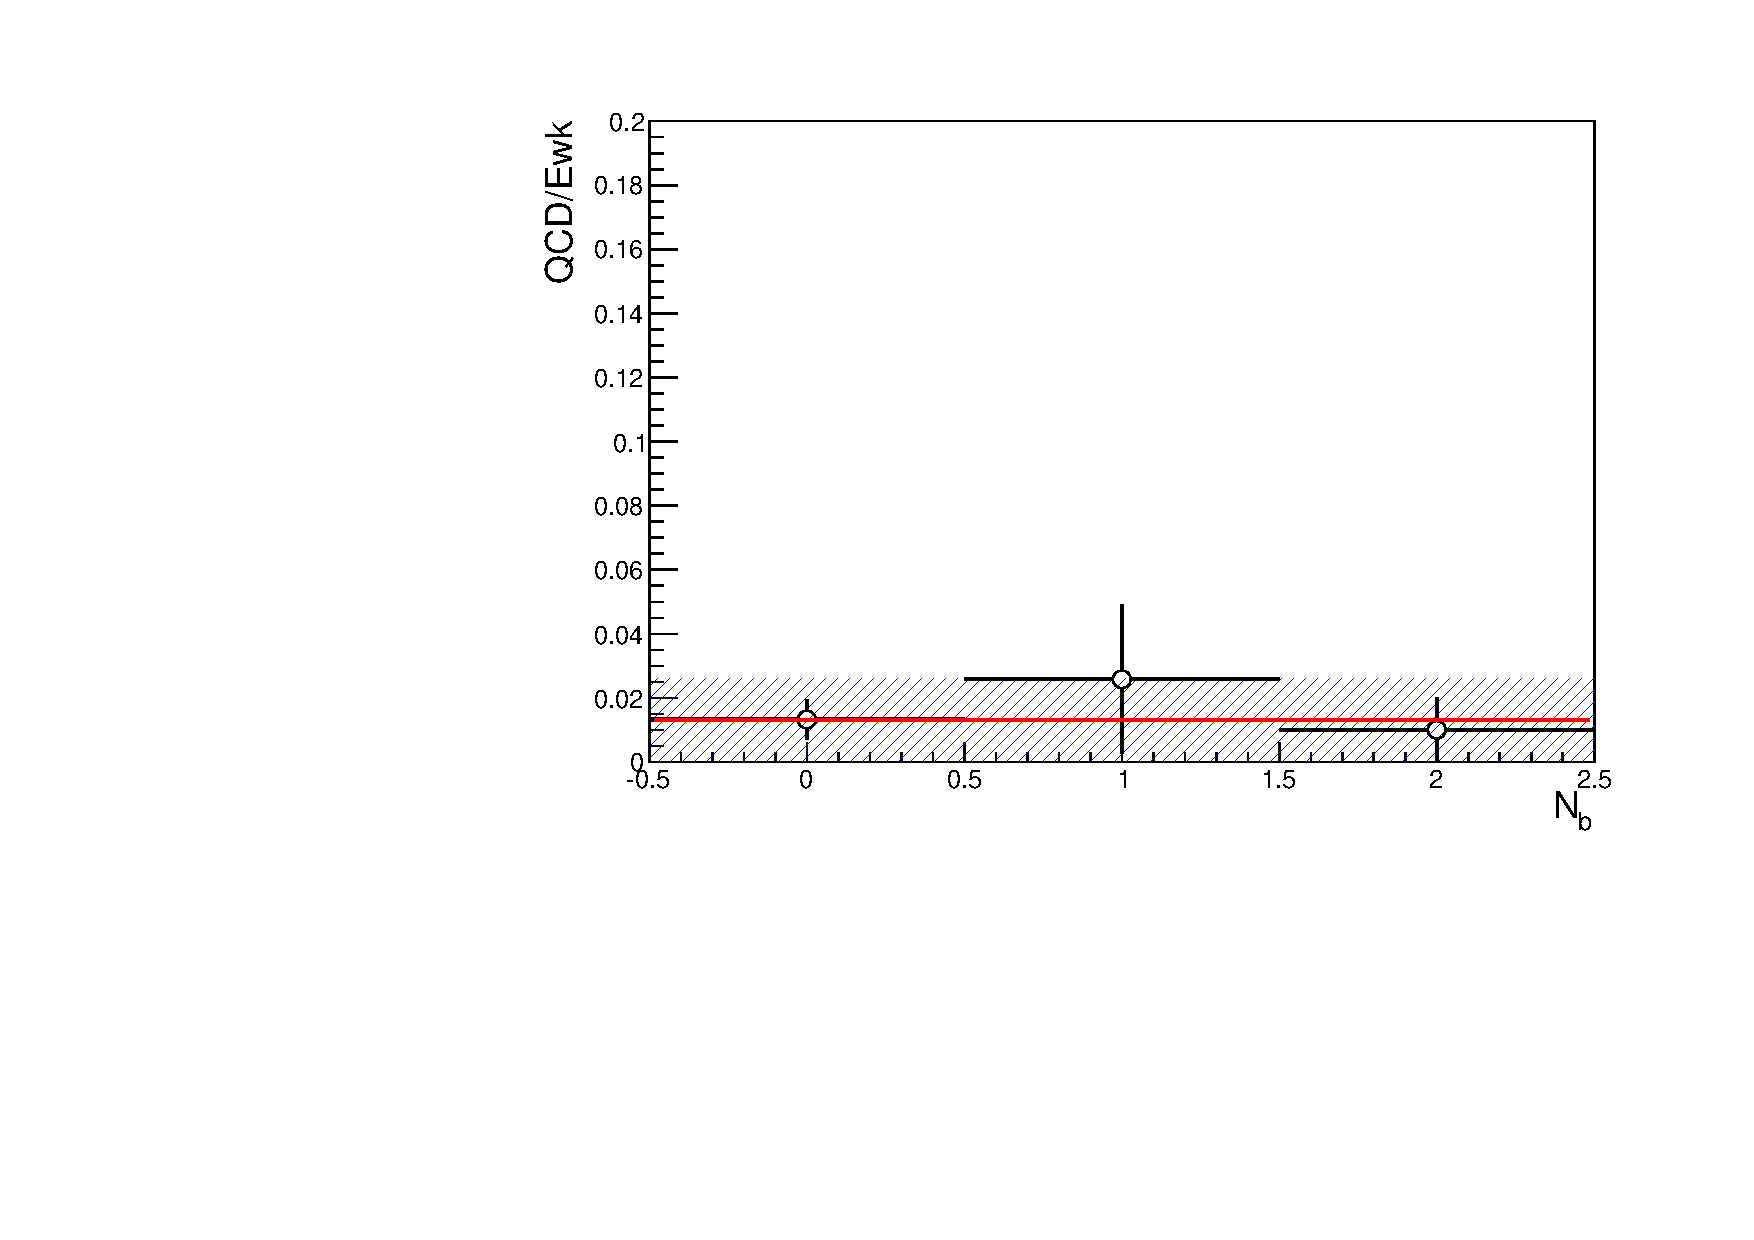
\includegraphics[width=0.5\textwidth]{figures/qcd/validation/Ratio_Sym_HTgt800_nB}} \\
      \caption{ Ratio of QCD to electroweak Monte Carlo prediction in the signal region for different \scalht selections as a function of \mht (Left) and $\nb$ (Right) for the asymmetric jet category. A constant fit to the data is represented by the red line, with the $\pm$100\% uncertainty represented by the blue hashed region.
    }
    \label{fig:sym_qcd_validation}
  \end{center} 
\end{figure}
